\documentclass{article}
\usepackage[thmmarks, framed]{ntheorem} % ntueorem must come before amsmath, or the cross-reference will not be working
\usepackage[utf8]{inputenc}
\usepackage{graphicx}
\usepackage{booktabs}
\usepackage[a4paper, portrait, margin=1in]{geometry}
\usepackage{amsmath}
\usepackage{amsfonts}
\usepackage{mathtools}
\usepackage{physics}
\usepackage{xcolor}
% needed for framed theorems
\usepackage{framed} % or, "mdframed"
%
\usepackage{bm}
\newcommand{\up}{\ket{\uparrow}} % spin up, needs the physics package 
\newcommand{\dn}{\ket{\downarrow}} % spin down, needs the physics package 
\newtheorem{theorem}{Theorem} 
\newframedtheorem{frm-thm}{Theorem} %needed for framed theorems 
\theorembodyfont{\upshape}
\newframedtheorem{frm-res}{Result}
\theorembodyfont{\upshape}
\newframedtheorem{frm-def}{Definition}
\theoremstyle{nonumberplain} 
\theoremheaderfont{\itshape}
\theorembodyfont{\normalfont}
\theoremsymbol{\ensuremath{\square}}
\newtheorem{proof}{Proof}
\title{Thermal Physics}
\author{Yu Lu}
\begin{document}
\maketitle
\section{Mathematical tricks}
A few important results from multivariate calculus include
\begin{itemize}
    \item Chain rule: useful for change of variable $U(x,y)$ into $U(u,v)$
    \[
        \left(\frac{\partial U}{\partial x} \right)_y = 
        \left(\frac{\partial U}{\partial u} \right)_v \left( \frac{\partial u}{\partial x} \right)_y
        + \left(\frac{\partial U}{\partial v} \right)_u \left( \frac{\partial v}{\partial x} \right)_y
    \]
    \item Reciprocal rules: useful for changing the subject variable (``dependent variable'')
    \[
        \begin{aligned}
            \left(\frac{\partial X}{\partial Y} \right)_Z &= \left(\frac{\partial Y}{\partial X} \right)_Z^{-1} \\
            \left(\frac{\partial X}{\partial Y} \right)_Z 
            \left(\frac{\partial Y}{\partial Z} \right)_X &
            \left(\frac{\partial Z}{\partial X} \right)_X = -1.
        \end{aligned}
    \]
\end{itemize}

The second reciprocal rule is often useful when a thermodynamic potential is held constant: we just turn it to the numerator. 

This allows us to easily navigate between differentials of different thermodynamic quantities, yet the question remains: what do we know about the quantities themselves? For example, we might know $p(V,T)$ and correspondingly
\[
    \left( \frac{\partial F}{\partial V} \right)_{T} = -p.
\]
The best we can do, then, is to integrate the differential with respect to $V$ and hold the $T$ constant:
\[
    F (V,T)
    = f(T) + \int \left( \frac{\partial F}{\partial V} \right)_{T} \mathrm{d} V
    = f(T) + \int -p(V,T) \mathrm{d} V, 
\]
leaving an undetermined function that only depends on $T$ and up to a constant. 

A ton of partial differentials can be generated from the algebra above, but often many of them have physical meanings or can be converted. For example, temperature derivatives of entropy can be associated with heat capacities:
\[
    \boxed{
    C_V = T \left(\frac{\partial S}{\partial T} \right)_V = \left(\frac{\partial U}{\partial T} \right)_V
    , \qquad 
    C_p = T \left(\frac{\partial S}{\partial T} \right)_p = \left(\frac{\partial H}{\partial T} \right)_p.}
\]

Thermodynamic variables are grouped into conjugate groups $\{V,p\},$ $\{S,T\},$ and $\{\mu ,N\}.$ The partial derivative of one thermodynamic variable with respect to another thermodynamic variable can be converted to another such partial differential using Maxwell's relations. Often, we want to convert such partial differentials into the conjugate pair $\{V,p\}$ in questions involving gas because the equation of state relates $V$ and $p$ to $T.$ A systematic approach can be used to spot which relation to use: say we start with 
\(
    \left( \frac{\partial S}{\partial p} \right)_{T}, 
\)
then thermodynamic potential we want to consider will have a total differnetial
\[
    \mathrm{d} B = \pm S \mathrm{d} T \pm x \mathrm{d} p, 
\]
where $B$ is a thermodynamic potential and $x$ is a thermodynamic variable. The potential of interest must then be $G$ with $\mathrm{d} G = -S\mathrm{d} T + V \mathrm{d} p,$ giving the Maxwell relation of interest
\[
    \left( \frac{\partial S}{\partial p} \right)_{T} = 
    -\left( \frac{\partial V}{\partial T} \right)_{p}. 
\]

The partial differential of a thermodynamic potential with respect to one thermodynamic variable could be identified as another thermodynamic variable. This is only true if the two are natural variables of the potential. For example, because \(\mathrm{d} G = -S\mathrm{d} T + V \mathrm{d} p,\) we can identify
\[
    \left( \frac{\partial G}{\partial T} \right)_{p} = -S, 
    \qquad
    \left( \frac{\partial G}{\partial p} \right)_{T} = V.
\]
\section{Phase Transition}
\subsection{Real gases}
Ideality of gas assumes that the gas molecules have no volumes and no intermolecular interactions. In reality, the long-range forces (van de Waals force, for example) drag the molecules together and the finite size of molecules reduces the available space for them to jiggle. We thus want to modify the ideal gas law $p_i V_{mi} = R T,$ where the subscript $m$ denotes molar quantity and $i$ denotes ideality. There are different phenomenological models to express $p_i$ and $V_{mi}$ using the measurable $p$ and $V_m$ (note that we assume them to be equal in the ideal gas law). 

To account for the finite size of molecule sizes, we simply let $V_i = V - b,$ where $b$ is a parameter to be fixed, making the available volume less than the actual volume of the container. The \textit{\textbf{van de Waals}} model of real gas accounts for the intermolecular attraction by $p_i = p + a/V_m^2,$ reducing the actual pressure by the long-range attraction. The $1 / V_m^2$ form of the pressure reduction can be rationalised by approximating the net interaction potential $U$ as proportional to the number of particles $\propto n$ multiplied by the number of nearest neighbouring paris $ \propto n/V$ with the strongest interaction: $U = -a n^2 /V$ The associated effective pressure ($p_i + p_{\mathrm{eff}} = p$) can be determined by $-p_{\mathrm{eff}} \mathrm{d}V = \mathrm{d} U,$ giving the equation of state 
\begin{equation}
    \label{eq:vdw-eq}
    \boxed{
        \left( p + \frac{a}{V_\mathrm{m}^2}\right) (V_\mathrm{m}  - b) = RT.
    }
\end{equation}

Eq.\eqref{eq:vdw-eq} cannot be solved explicitly (easily) for $V$, but it is relatively easy to give an explicit expression for $p$ as 
\[
    p(V,T) = \frac{RT}{V-b} - \frac{a}{V^{2}.}
\]
Often we want to use $p$ as our ``subject variable'' by performing the relevant math trick. For example, 
\[
    \left( \frac{\partial V}{\partial p} \right)_{T} = 
    \left( \frac{\partial p}{\partial V} \right)_{T} ^{-1}.
\]

Various thermodynamic quantities can be obtained from Eq.\eqref{eq:vdw-eq} from chain rules and the Maxwell relations. For example, the entropy is
\[
    \begin{aligned}
        \mathrm{d}S &= \left(\frac{\partial S}{\partial T}  \right)_V \mathrm{d}T + \left(\frac{\partial S}{\partial V}  \right)_T \mathrm{d}V  \\
        &= \frac{C_V}{T}\mathrm{d} T + \left(\frac{\partial p}{\partial T}  \right)_V \mathrm{d}V,
    \end{aligned}
\]
where the second line follows from a Maxwell's relation. The equation of state for a van de Waals gas then gives
\[
    S = C_V \ln T + R \ln (V -b) + \mathrm{const},
\]
which is independent of $a$ since entropy only cares about the allowed space for different configurations. We can also evaluate 
\[
    \Delta U = a \left( \frac{1}{V_1} - \frac{1}{V_2}\right),
\]
which is independent of $b$ since it only cares about intermolecular interactions. 

\subsection{Phase transition of gas to liquid}
Eq.\eqref{eq:vdw-eq} is in general cubic in $V,$ as shown in Fig.\ref{fig:vdw-isotherm}, so the isotherms might adopt an S-shaped curve with two extrema. This isn't allowed in \textit{equilibrium} thermodynamics, as the isothermal compressibility 
\[
    \kappa_T = - \frac{1}{V}\left(\frac{\partial V}{\partial p} \right)_T
\]
should always be positive. This means a positive fluctuation in $p$ expands the gas, making it unstable in a positive feedback loop. At equilibrium, the Gibbs free energy would always be minimised in a constant pressure and temperature experiment, moving along $ABC$ in the $G-p$ plot. The turning point $B$ corresponds is multivalued in the $V-p$ plot and can thus be interpreted as \textit{two phases in equilibrium}: the one on the branch with large volume and large compressibility is gas and the other is liquid. It is worth reiterating that this \textit{\textbf{phase transition}} does not emerge in the ideal gas assumption because intermolecular interaction, which is neglected in gas, cannot be neglected in liquid. 

\begin{figure}[ht]
    \centering
    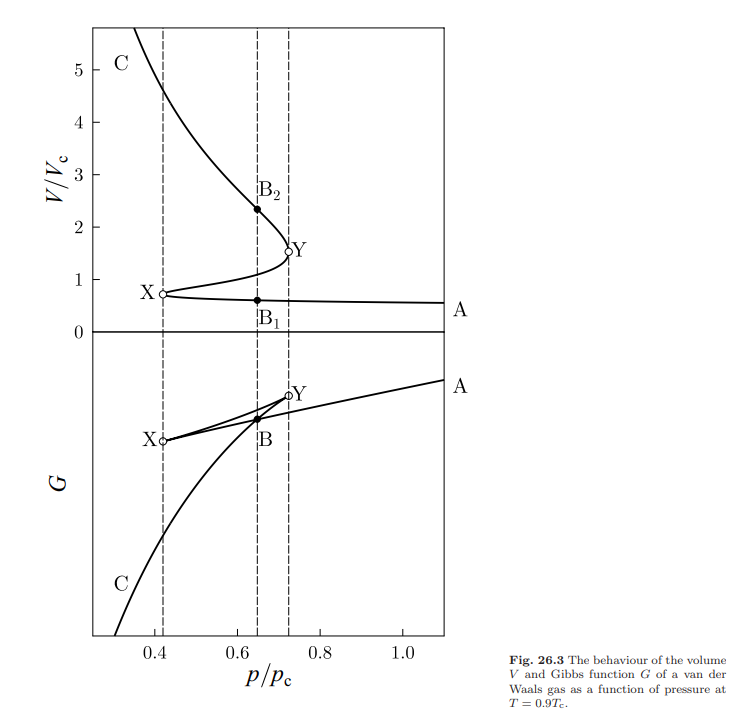
\includegraphics[width=0.8\textwidth]{fig/Blundell-p301.png}
    \caption{Sub-critical van de Waals isotherm. The kinetically feasible path $AXYC$ is different from the thermodynamically stable path $AB_1B_2C$ (Blundell and Blundell, p.p.301)} 
    \label{fig:vdw-isotherm}
\end{figure}

At the transition point $B,$ the Gibbs energy has a double well profile (corresponding to the gas and liquid) with equal depth in the phase space, which becomes biased as one deviates from the equilibrium pressure or volume of coexistence. As one contracts the gas, the gas is stuck at the shallower well that is closer to its original gaseous phase going past the equilibrium volume, giving rise to supercooling along $CY.$ The equilibrium is prevented because of an energy barrier between the two phases and the gas is in a \textit{\textbf{metastable phase}}. However, once a perturbation energy is given, the supercooled gas will return to the equilibrium gas phase, corresponding to a vertical line in the phase diagram. Note that only at $B$ can there be two phases coexisting at equilibrium, and supercooling/superheating are just metastable phases with a higher Gibbs free energy. 

The critical point for phase transition $B$ can be determined by the single-valuedness of $G$ at this point: $G(B_1) = G(B_2). $ Since $G$ is also state function with $V = (\partial G / \partial p )_T$, the change in $G$ along $B_1XYB_2$ must also be 0: 
\[
    \int_{B_1}^{B_2} V  \,\mathrm{d}p =0,
\]
giving the \textit{\textbf{Maxwell construction of equal area}}.  

The coordinates (p, V, T) at the coexistence point $B$ can be used to plot a phase diagram for the gas and liquid. However, the occurrence of a phase transition requires the $S$-shaped profile of isotherms in the first quadrant, which is only feasible up to a critical $T_\mathrm{c},$ mathematically determined by finding the point of inflexion of the isotherm:
\[
    \boxed{
        \left. \left(\frac{\partial p}{\partial V} \right)_T  = 0 \, \right \vert_{T= T_c}, \qquad
        \left. \left(\frac{\partial^{2}  p}{\partial V^{2} } \right)_T  = 0 \, \right \vert_{T= T_c}
    }
\]
There is no phase transition at a higher temperature and the distinction between phases ceases to exist, giving supercritical liquids.

There are other phenomenological models of the real gas. For example, the Dieterici equation takes the boltzmann distribution into consideration, giving 
\[
    p (V_m - b) = RT \mathrm{\exp } \left( -\frac{a}{RT V_\mathrm{m} }\right).
\]

A useful quantity to test ideality is the compressibility factor 
\[
    Z = \frac{pV_\mathrm{m} }{RT}, 
\]
which is unity for the ideal gas. At the critical point, $Z = 3 /8$ for van de Waals gas and $Z \approx 0.27 $ for Dieterici gas. 

Motivated by this factor, we can also model real gas via the virial expansion 
\[
    Z = 1 + \frac{B^\prime }{V_\mathrm{m}  } + 1 + \frac{C^\prime }{V_\mathrm{m}^2  } + \ldots  
    = 1 + \frac{B(T)}{V_\mathrm{m} }, 
\]
where the infinite power series can be terminated at the first term by giving $B(T)$ a temperature dependence. $B = 0$ for an ideal gas, but there is a finite temperature $T_\mathrm{B} $ (called the \textit{\textbf{Boyle temperature}}) at which $B = 0$ again (this is a result of the Leonard-Jones potential). 

\subsection{The law of corresponding states}
The empirical parameters $a$ and $b$ in van de Waals equation differ from gas to gas, but the gas's property can be fully specified by the position and depth of the potential well. Therefore, all gases are the same in the reduced phase coordinates $V/V_c$, $p / p_c$ ,and $T / T_c$ (two degrees of freedom for the intermolecular interaction and one more for the sizes of the particles). However, the quantum mechanical effects prominent in hydrogen and helium breaks this law. 
\subsection{Cooling real gases: Joule-Kelvin expansion}
Ideality of the gas assumes that its internal energy $U$ only depends on the temperature $T$. For an ideal gas, its temperature does not change during a Joule expansion which is adiabatic with no external work, giving 
\[
    \boxed{
    \mu_J \equiv \left(\frac{\partial T}{\partial V} \right)_U 
    = -\frac{1}{C_V} \left( \frac{\partial U}{\partial V} \right)_T}
    = -\frac{1}{C_V} \left[ T \left(\frac{\partial p}{\partial T} \right)_V - p\right]= 0.
\]
For a van de Waals gas, however, it will cool during expansion with 
\[
    \mu_J = -\frac{a}{C_V V^2}, \implies \Delta T = -\frac{a}{C_V} \left( \frac{1}{V_1} - \frac{1}{V_2}\right) <0
\]
Similarly, an \text{isothermal} expansion of van de Waals gas increases its potential energy as 
\[
    \Delta U = a \left(\frac{1}{V_1} - \frac{1}{V_2}\right) >0.
\]

Cooling via Joule expansion is not useful in practice, and we're interested in a constant-enthalpy flow process, thus defining the Joule-Kelvin coefficient 
\[
    \mu_{\mathrm{JK}} = \left(\frac{\partial T}{\partial p}\right)_H. 
\]
From a similar manipulation as that for the Joules coefficient, 
\[
    \mu_{\mathrm{JK}} = -\frac{1}{C_p} \left(\frac{\partial H}{\partial p} \right)_T
    = \frac{1}{C_p} \left[ T\left(\frac{\partial V}{\partial T} \right)_p - V\right]
\]
which can be either positive or negative, though the entropy change is positive definite. Whether we get a cooling or heating from the Joule-Kelvin expansion depends on the exact $p$ and $T,$ but there is a maximum temperature for cooling to happen, known as the \textit{\textbf{inversion temperature}}, below which it is feasible to cool the gas by throttling like this.  

The inversion temperature $T_C$ is the temperature at which $\mu_{\mathrm{JK} } =0,$ determined by 
\[
    T \left( \frac{\partial V}{\partial T} \right)_{p} - V= 0
    \implies 
    -\frac{\left( \frac{\partial p}{\partial T} \right)_{V} }{\left( \frac{\partial p}{\partial V} \right)_{T} } = \frac{V}{T}.
\] 
This is a curve for a real gas with a maximum inversion temperature above which the Joule-Kelvin flow process only heats the gas. But for a van de Waals gas, the inversion temperature is $T_C = 2 T_B$, a constant at all pressure, where $T_B$ is the Boyle temperature ($T_B = \frac{a}{b R}$ for a van de Waals gas).

In practice, we can liquefy different gas in a sequence, starting with the species with highest inversion temperature. In the flow process, high-pressure gas is injected while liquid and gas at atmospheric pressure is ejected. The maximum efficiency of liquefaction occurs when 
\[
    \left(\frac{\partial H_{\mathrm{in}}}{\partial p_\mathrm{in}}  \right)_{T_\mathrm{in}} = 0,
\] along the inversion temperature line with $\mu_{\mathrm{JK} } = 0,$ echoing the line that maximum efficiency is gained only in a reversible process. 

\subsection{Phase Transition}
Heat capacity and latent heat
stable phase minimises Gibbs free energy 
near the triple point, the L of sublimation of L of fusion + L of vaporization 
Clausius-Clapeyron for all three transitions (approximations made). ideal phase diagram
Integration: assuming constant L or not
the gibbs phase rule and phase transition classification

\end{document}